\chapter{Introduction}

\TODO{Recapitulate main points of project thesis:}

\TODO{some general intro about the possibility of quark stars}

In this chapter, we will study a hypothetical class of compact stars known as quark stars.
Let us summarize the main ingredients in this work.

\section{Tolman-Oppenheimer-Volkoff equation}

In \cref{chap:tov} we derived the Tolman-Oppenheimer-Volkoff equation
\begin{subequations}
\begin{align}
	\odv{P}{r} &= -\frac{G m \epsilon(P)}{r^2 c^2} \left( 1 + \frac{P}{\epsilon(P)} \right) \left( 1 + \frac{4 \pi r^3 P}{m c^2} \right) \left( 1 - \frac{2 G m}{r c^2} \right)^{-1} , \\
	\odv{m}{r} &= \frac{4 \pi r^2 \epsilon(P)}{c^2} .
\end{align}
\end{subequations}
It determines the pressure and mass gradients with relativistic corrections inside a spherically symmetric star composed of a perfect fluid in hydrostatic equilibrium.
Given the fluid's equation of state $\epsilon(P)$ that relates its pressure $P$ to its energy density $\epsilon$, it is a system of two equations for the two unknowns $P$ and $m$ and can be integrated.
We will seek mass-radius solutions to the equation, obtained by integrating it from the center $r=0$ with zero initial mass $m(0) = 0$ and some central pressure $P(0) = P_c$ until reaching the surface $r=R$ defined by a vanishing pressure $P(R) = 0$ and where the mass $m(R) = M$ defines the star's total mass.
By finding such solutions for a range of central pressures $P_c$, we parametrize a sequence of stars that we can plot in a mass-radius diagram.

\section{Thermal field theory}

To derive equations of state for quark matter, we will study quantum field theories whose dynamics is described by some Lagrangian density $\lagr$.
In \cref{chap:tft} we showed that the partition function in the grand canonical ensemble corresponding to a Lagrangian including both a fermionic field $\psi$ and a bosonic field $\phi$ is given by the path integral
\begin{equation}
	Z = \oint_- \pathintdif \bar{\psi} \oint_- \pathintdif \psi \oint_+ \pathintdif \phi \exp \Big\{ \int_0^\beta \dif \tau \int_V \dif^3 x \, \lagr_E[\bar{\psi}, \psi, \phi] \Big\} = e^{-\beta V \Omega} .
\end{equation}
Here $V$ is the spatial volume of the system, while its inverse temperature $\beta = 1/T$ define its ``temporal'' extent.
The sign subscripts on the closed integral signs is supposed to remind us of a property we showed extensively in \cref{chap:tft}: the bosonic fields must be periodic in inverse temperature time, while the fermionic fields must be anti-periodic.
If a symmetry of the Lagrangian admits a conserved Noether charge density $j^0$, we also saw that we could couple it to a chemical potential $\mu$ in the Lagrangian by including the term $\mu j^0$.
By computing (the logarithm of) the partition function, we have the grand potential $\Omega = -\log Z / \beta V$ from which we can calculate all thermodynamic quantities such as the (mean)
\TODO{this is already in $T=0$ form? write in general $T \geq 0$ form in this intro?}
\begin{equation}
	\text{density} \quad n = -\pdv{\Omega}{\mu}, \quad
	\text{pressure} \quad P = -\Omega, \quad
	\text{energy density} \quad \epsilon = -P + \sum_p \mu_p n_p .
\end{equation}
These expressions are valid in the approximation of zero temperature $T=0$ that we saw was valid for neutron stars in \cref{chap:nstars}.
As quark stars are expected to be ``more intense neutron stars'', we assume that this approximation still holds.

The equation of state $\epsilon(P)$ follows by eliminating the chemical potentials $\mu_p$ from the energy density $\epsilon(\mu_p)$ in favor of the pressure $P$.
In \cref{chap:nstars} we did so for pure neutron stars, for which there was only one chemical potential to eliminate.
Now we will study quark stars composed of up quarks, down quarks, strange quarks and electrons, each associated with their own chemical potential $\mu_p$.
With these \emph{four} particles, we require \emph{three} additional relations that reduce the dependence of the pressure and energy density to \emph{one} independent chemical potential, which can finally be eliminated to yield the equation of state.

\subsubsection{Chemical equilibrium of weak interaction processes}

We can obtain two relations between the chemical potentials by studying the nuclear processes that take place inside the star.
According to \cite{ref:quark_star_processes}, quarks stars may be formed as hadronic matter in a neutron star decays to strange quark matter through weak interactions processes like
\begin{equation}
	u + e^- \rightarrow d + \nu_e
	\qquad \text{and} \qquad
	u + e^- \rightarrow s + \nu_e .
\end{equation}
Over time, the star cools and neutrinos diffuse out. \cite[section 5.3]{ref:glendenning}
We therefore set $\mu_{\nu_e}=0$, so that the chemical equilibrium of the two processes above implies
\begin{equation}
	\mu_d = \mu_s = \mu_u + \mu_e .
\label{eq:lsm:chemical_equilibrium}
\end{equation}
These are the two announced relations between the four chemical potentials.

\subsubsection{Electric charge neutrality of stars}

The third and last additional relation relating the four chemical potentials is provided by electric charge neutrality.
We can make a strong and simple classical argument for why there can be no \emph{global} net electric charge in stars by comparing Newton's law of gravity and Coulomb's law.
Consider a test particle of mass $m$ and electric charge $q$ on the surface $R$ from the center of a star with total mass $M$ and electric charge $Q$.
In an idealized situation, the test particle is affected by the gravitational and electrostatic force, so that the total outwards radial force on it is
\begin{equation}
	F_\text{out} = -G \frac{M m}{R^2} + k_e \frac{Q q}{R^2} .
\end{equation}
Furthermore, suppose the star consists of a great number $N$ of particles weighing, each with mass $m < m_B$ that is lower than some heavy baryon mass $m_B$ and about one elementary charge $q \approx \pm e$.
We then have $M < N M_B$ and $m < m_B$.
If the star had an opposite charge $Q = \mp Z e$, then $F_\text{out} < 0$ and the test particle would stay in the star, seeking to neutralize it.
On the other hand, if the star has a like charge $Q = \pm Z e$, then
\begin{equation}
	F_\text{out} > -G \frac{N m_B^2}{R^2} + k_e \frac{Z e^2}{R^2} .
\end{equation}
Assuming a typical baryon mass $m_B = m_p = \SI{1.67e-27}{\kilogram}$,
we then surely have $F_\text{out} > 0$ provided that the number of elementary charges per particle satisfies
\begin{equation}
	\frac{Z}{N} > \frac{G m_B^2}{k_e e^2} \approx 10^{-37} .
\end{equation}
This means that particle are expelled from the star while $Z > 10^{-37} N$ until $Z$ has fallen to \emph{at least} $Z < 10^{-37} N$.
We conclude that for all practical purposes, stars are \emph{globally} electrically charge neutral.
As explained by \cite{ref:master_halvor}, this argument is slightly modified by relativistic corrections, but the conclusion is not.

In a star that consists of a set of particles $p$ each with charge $q_p$, we could implement \emph{global} charge neutrality by constraining the chemical potentials such that the charge density
\begin{equation}
	\sum_p q_p \, n_p(\mu_p) = \rho(r)
\label{eq:intro:charge_neutrality_global}
\end{equation}
at radius $r$ is equal to some charge density function $\rho(r)$ that causes the total charge $Q = \int \rho(r) 4 \pi r^2 \dif r = 0$ \TODO{add relativistic correction $e^{\beta(r)}$ from metric?} to vanish.
This approach would make the equation of state $\epsilon(P,r)$ dependent on radius in addition to pressure.
It is not obvious how one should single out one of the infinitely many possible charge density profiles $\rho(r)$.
We will avoid this problem altogether by rather assuming that charge neutrality holds \emph{locally} with $\rho(r) = 0$.
Then the equation of state $\epsilon(P)$ is again a function of pressure only, obtained by eliminating chemical potentials according to
\begin{equation}
	\sum_p q_p \, n_p(\mu_p) = 0
\label{eq:lsm:charge_neutrality}
\end{equation}
As shown in \cite{ref:global_neutrality}, for example, this simplification can modify the masses and radii of stars within an order of magnitude, but the differences are smaller closer to the maximum mass star.
In fact, \cite{ref:local_neutrality_inconsistent} has shown that local charge neutrality in neutron stars composed of protons, neutrons and electrons is unphysical.
Our choice $\rho(r)=0$ is therefore the simplest choice, but not the most physical one.

\section{Quantum chromodynamics}

The theory of the strong interaction force is called \textbf{quantum chromodynamics} (\textbf{QCD}).
It describes the interaction between quarks mediated by gluons through the Lagrangian density
\begin{equation}
	\lagr = \bar{q} ( i \gamma^\mu D_\mu - m ) q - \frac14 G_{\mu\nu}^a G^{\mu\nu}_a
	\qquad \text{with} \qquad
	G_{\mu\nu}^a = \partial_\mu A_\nu^a - \partial_\nu A_\mu^a + g f^{abc} A_\mu^b A_\nu^c.
\label{eq:qcd:lagrangian}
\end{equation}
The quark fields $q = q_{f,c,\alpha}(x)$ are indexed by
the $N_f = 3$ flavors $f \in \{u,d,s\}$,
the $N_c = 3$ colors $c \in \{r,g,b\}$ and
$4$ Dirac spinor indices $\alpha \in \{0,1,2,3\}$,
and we will take a flavor index $f$ with the shorthand $f = q_{f,c,\alpha(x)}$.
The gamma matrices \eqref{eq:tft:gamma_dirac_basis} act in spinor space,
the mass matrix $m = \diag(m_u, m_d, m_s)$ in flavor space,
and there are suppressed identity matrices in spinor, flavor and color space wherever needed for the Lagrangian to be a scalar.
The covariant derivative is $D_\mu = \partial_\mu - i g A_\mu^a T^a$ and couples the gluon gauge fields $A_\mu^a$ to the quarks with strength $g$.
Finally, the Gell-Mann matrices $T^a$ are the $N_a = N_f^2 - 1$ generators of the symmetry group $SU(N_f)$,
whose structure constants $f^{abc}$ can be determined from the commutators $\comm{T^a}{T^b} = i f^{abc} T^c$.

\TODO{mention it is a Yang-Mills theory?}
\TODO{derive (in a plausible way) by generalizing QED?}

\subsubsection{Phase diagram and calculational methods}

\begin{figure}[t]
\centering
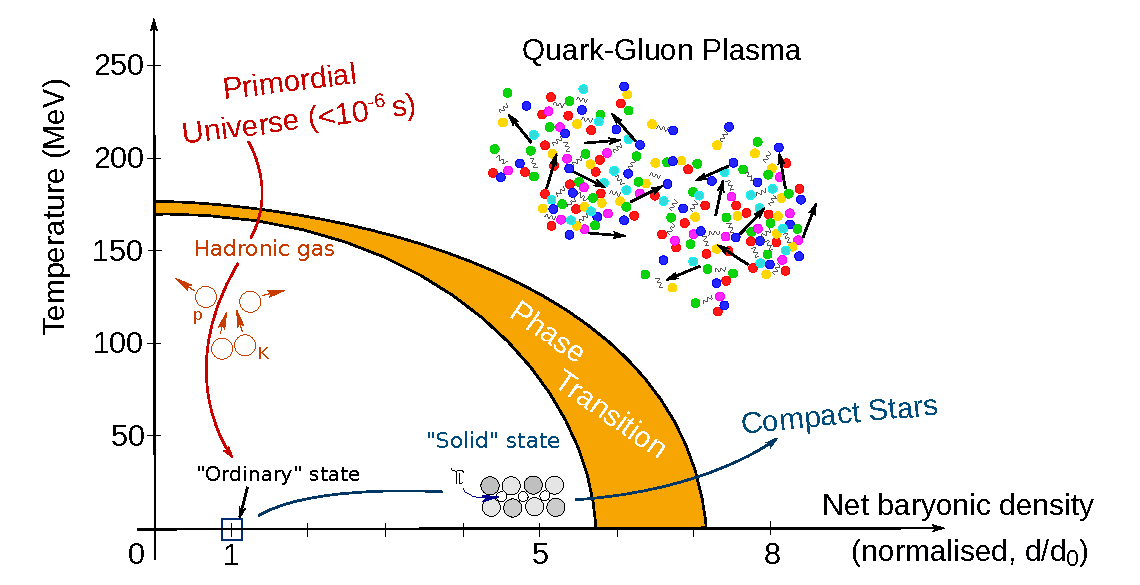
\includegraphics[width=0.9\textwidth]{figures/qcd-phase-diagram.pdf}
\caption{%
	Slice of the phase diagram of quantum chromodynamics with zero isospin and strangeness.
	\credit{CERN / Antonin Maire}{https://cds.cern.ch/record/2025215}
}
\label{fig:qcd:phase_diagram}
\end{figure}

The phase diagram of quantum chromodynamics describes the phase of quark matter as a function of temperature $T$, the quark chemical potential $\mu_Q$, the isospin chemical potential $\mu_I$ and the strangeness chemical potential $\mu_S$.
Although mapping out the diagram is an active area of research, a rough qualitative picture is known, and the slice with $\mu_I = \mu_S = 0$ is shown in \cref{fig:qcd:phase_diagram}.
Later we will see that the state of matter in compact stars is parametrized by a curve in the phase diagram that lies close to the $\mu_Q$-axis, corresponding to the density of baryons.
We will shortly discuss the most important qualitative properties of quantum chromodynamics and relate them to this phase diagram.

Quantum chromodynamics is notorious for being very difficult to make analytical calculations with, and its elegance and practicality stops not longer after writing down its Lagrangian \eqref{eq:qcd:lagrangian}.
To explore the phase diagram, one must therefore resort to alternative techniques:
\begin{itemize}
\item \textbf{Perturbation theory} can be used to study quantum chromodynamics at \emph{high} energy, perhaps contrary to what one might expect.
      As we will soon discuss in more detail, this is due to a property called asymptotic freedom that causes the interaction strength to \emph{decrease} with increasing energy.
\item \textbf{Lattice QCD} consists of making numerical calculations on a discrete lattice of spacetime points.
      This method has proved very useful for studying quantum chromodynamics under quite general circumstances.
      In the regime of high density and low temperature, however, is plagued by the so-called sign problem that refers to the difficulty of calculating integrals of highly oscillatory functions.
      This is precisely the area in the phase diagram that is relevant for compact stars.
\item The \textbf{$\bm{1/N_c}$-approximation} or \textbf{large $\bm{N_c}$-limit} consists of making expansions in the assumed small parameter $1/N_c$.
      Although there are only $N_c = 3$ colors in nature, this scheme has indeed been used to make accurate predictions.
      We will refer to this approximation to justify some of our later actions.
\item \textbf{Effective theories and models} can be used to study quantum chromodynamics in some regimes of interest.
      The most important requirements of such a theory or model is that it includes the correct degrees of freedom (or particles) and exhibit the same symmetries and symmetry breaking patterns as the theory it aims to describe in the regime of interest.
      Due to \cite{ref:weinberg_eft}, the philosophy is then to ``write down the most general possible theory involving fields for these particles, including all possible interactions consistent with the symmetries''.
      For example, chiral perturbation theory ($\chi$PT), the Nambu-Jona-Lasinio (NJL) model and the linear sigma model (LSM), also known as the quark-meson (QM) model, all give effective descriptions of quantum chromodynamics at low energies.
      This approach is applicable to compact stars and is the one we will take.
\end{itemize}

\subsubsection{Color confinement and asymptotic freedom \cite{ref:quark_bag_model}}

\begin{figure}
\centering
\tikzsetnextfilename{bag-model}
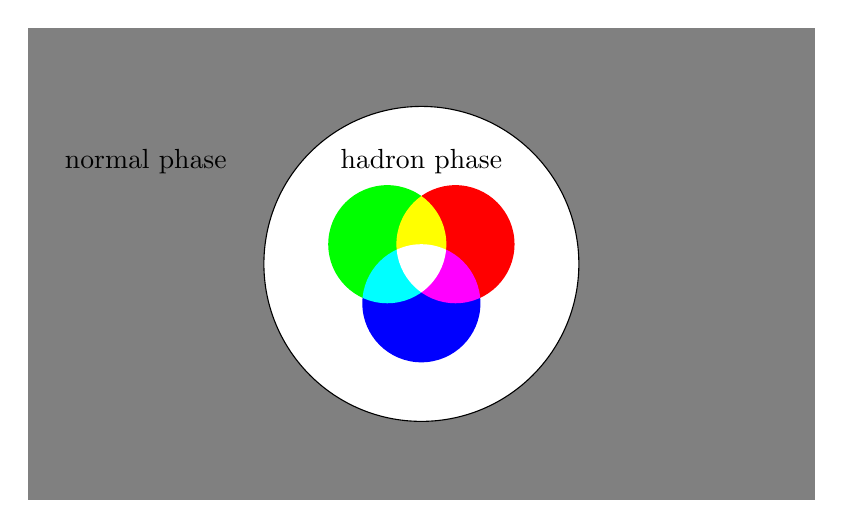
\begin{tikzpicture}
\fill [gray] (-5, -3) rectangle (+5, +3);

\draw [draw=black, fill=white] (0, 0) circle (2);
\begin{scope}[blend group=screen]
	\fill [fill=red]   (30:0.5)  circle (0.75) node {$u$};
	\fill [fill=green] (150:0.5) circle (0.75) node {$d$};
	\fill [fill=blue]  (270:0.5) circle (0.75) node {$s$};
\end{scope}
\node at (90:1.3) {hadron phase};
\node at (-3.5,1.3) {normal phase};
\end{tikzpicture}
\caption{\label{fig:lsm:confinement}%
	\TODO{caption}
}
\end{figure}

One fundamental feature of quantum chromodynamics is \textbf{color confinement}.
Quarks can be color-charged \textcolor{red}{\textbf{red}}, \textcolor{green}{\textbf{green}} and \textcolor{blue}{\textbf{blue}},
while antiquarks can have the complementary anticolors \textcolor{cyan}{\textbf{antired}}, \textcolor{magenta}{\textbf{antigreen}} and \textcolor{yellow}{\textbf{antiblue}}.
At low temperature and density, experiments and lattice simulations show that quarks never appear in isolation, but are always confined in hadrons that have no overall color.
As the distance between color-charged quarks increases, the strong force between them remains \emph{constant} -- the quarks are  effectively ``glued'' together by the mediating gluon.
For example, a meson consists of one quark of any color and one antiquark of its complementary color, making the meson itself colorless or ``white''.
Similarly, a(n) (anti)baryon consists of one (anti)red, one (anti)green and one (anti)blue quark and is also ``white''.

What if an even stronger force overcomes the strong force and tries to forcibly separate the quarks in a hadron into colorful groups of quarks?
Then nature will simply create new quark--anti-quark pairs so that the new groups of quarks both become new colorless hadrons.
\TODO{Figure} illustrates this process for a meson.
At low temperatures and densities in the lower left of \cref{fig:qcd:phase_diagram}, quarks are therefore \emph{confined} in colorless hadronic matter that make up the present world around us.

In the opposite extreme, quantum chromodynamics displays the property of \textbf{asymptotic freedom}.
As the energy scale of quark interactions increases, or equivalently its length scale decreases, the interaction strength \emph{decreases}.
When the density reaches extreme levels, confined hadronic quark matter then turns into a \emph{deconfined} \textbf{quark-gluon plasma} in the upper right of \cref{fig:qcd:phase_diagram} where they are free of all interactions and move around at will.
It is believed that the universe passed through this phase during the first $\SI{20}{\micro\second}$ after the Big Bang, after which it transitioned to the present phase of hadronic matter.
As no human-made laboratory can possibly recreate the necessary densities in the near future, the best candidates for finding and studying this exotic state of matter today is precisely the cores of compact stars.
Asymptotic freedom was first discovered by \cite{ref:asymptotic_freedom_gross_wilczek,ref:asymptotic_freedom_politzer}, who were recognized with the Nobel Prize in 2004.

\subsubsection{Vector, axial and chiral symmetries and chiral symmetry breaking}

The Lagrangian \eqref{eq:qcd:lagrangian} has some interesting global symmetries, each of which gives rise to a conserved classical current by Noether's theorem.
The simplest symmetry is the $U(1)_V$ \textbf{vector symmetry} $q \rightarrow e^{i \theta} q$, giving rise to the conserved vector current $j^\mu = \bar{q} \gamma^\mu q$ representing the baryon number density.
In the grand canonical ensemble, we will later couple one such conserved current to a chemical potential for each quark flavor.
In the massless case $m = 0$, the Lagrangian also has the $U(1)_A$ \textbf{axial symmetry} $q \rightarrow e^{i \theta \gamma^5} q$ with the conserved axial current $j^\mu = \bar{q} \gamma^\mu \gamma^5 q$.
As its proof assumes the action to be extremized, Noether's theorem is inherently \emph{classical}.
Unlike the vector current, the axial current is no longer conserved under the influence of quantum effects, and is therefore said to be \emph{anomalous}.

Using the projection operator $P_\pm = \frac12 (1 \pm \gamma^5)$, we can introduce the left-handed ($-$) and right-handed ($+$) chiral fields $q_\pm = P_\pm q$.
One can then show that $q = q_- + q_+$, $\bar{q}_\pm q_\pm = 0$ and $\bar{q}_\pm \gamma^\mu D_\mu q_\mp = 0$, so that the Lagrangian \eqref{eq:qcd:lagrangian} can be written
\begin{equation}
	\lagr = \bar{q}_- i \gamma^\mu D_\mu q_- + \bar{q}_+ i \gamma^\mu D_\mu q_+ - \bar{q}_- m q_+ - \bar{q}_+ m q_- - \frac14 G_{\mu\nu}^a G^{\mu\nu}_a.
\label{eq:qcd:lagrangian_chiral}
\end{equation}
In the massless case $m=0$,
it is left invariant under the $SU(N_f)_L \times SU(N_f)_R$ \textbf{chiral symmetry} transformation $q_\pm \rightarrow U_\pm q_\pm$ where both $U_\pm \in SU(N_f)$.
Moreover, it is known that the ground state of quantum chromodynamics admits a nonzero quark condensate \cite[chapter 28]{ref:schwartz}
\begin{equation}
	\avg{\bar{q} q} %= \avg{\bar{q}_- q_-} + \avg{\bar{q}_+ q_+} + \avg{\bar{q}_- q_+} + \avg{\bar{q}_+ q_-}
	                                                            = \avg{\bar{q}_- q_+} + \avg{\bar{q}_+ q_-},
\end{equation}
which is generally \emph{not} invariant under the chiral transformation.
The fact that the ground state does not carry the same symmetry as its Lagrangian is the signature of \textbf{spontaneous symmetry breaking}.
Only if $U_- = U_+$ are all terms invariant -- this is the $SU(N_f)_V$ \textbf{isospin symmetry} where both left-handed and right-handed fields are transformed in the same way.
The isospin symmetry is also a symmetry of the \emph{massive} Lagrangian \eqref{eq:qcd:lagrangian_chiral} \emph{if} all quark masses are set equal so that the mass matrix $m$ proportional to the identity matrix.
We therefore say that quantum chromodynamics exhibits \textbf{chiral symmetry breaking}
\begin{equation}
	SU(N_f)_L \times SU(N_f)_R \quad (m = 0) \qquad \rightarrow \quad SU(N_f)_V \quad (m \neq 0).
\end{equation}
Goldstone's theorem then predicts that one massless Goldstone boson arises from every broken symmetry generator.
Hence, chiral symmetry breaking gives rise to $2 \times (N_f^2 - 1) - (N_f^2 - 1) = N_f^2 - 1$ Goldstone bosons.
With $N_f = 2$ and $N_f = 3$ flavors, these are the three pions and the eight light pseudoscalar mesons.

In the real world, however, the quarks have different masses and cause the chiral symmetry to be only \emph{approximately} broken.
We say that the different quark masses cause \textbf{explicit symmetry breaking}, in the sense that the Lagrangian changes by a small amount under the chiral transformation.
The physical consequence of this is that there are no massless Goldstone bosons, but rather very light pseudo-Goldstone bosons.

The breaking of chiral symmetry leads to the \textbf{chiral phase transition} colored orange in \cref{fig:qcd:phase_diagram},
connecting the phases of hadronic quark matter and quark-gluon plasma.


\pagebreak
\TODO{move below to LSM discussion?}

Quark-meson model can be written in terms of left/right fields:
\begin{equation}
\begin{split}
	\bar{\psi} \phi_5 \psi &= \bar{\psi} ( (P_+ + P_-) \sigma + (P_+ - P_-) i \tau \cdot \pi) \psi \\
	                       &= \bar{\psi} ( P_+ (\sigma + i \tau \cdot \pi) + P_- (\sigma - i \tau \cdot \pi) ) \psi \\
	                       &= \bar{\psi} ( P_+ \phi + P_- \phi^\dagger) \psi \\
	                       &= \bar{\psi} ( P_+ \phi P_+ + P_- \phi^\dagger P_-) \psi \\
	                       &= \bar{\psi}_- \phi P_+ + \bar{\psi}_+ \phi^\dagger \psi_- \\
\end{split}
\end{equation}
Used that $P_\pm^2 = P_\pm$ is in spinor-space, while $\phi$ is in flavor space.
Denote $+ = R$, $- = L$.
Now it is apparent that LSM is invariant under $SU(2)_L \times SU(2)_R$:
\begin{equation}
	\psi_+ \rightarrow U_+ \psi_+, \qquad
	\psi_- \rightarrow U_- \psi_-, \qquad
	\phi   \rightarrow U_- \phi U_+^\dagger.
\end{equation}
When $h \neq 0$, this symmetry is explicitly broken.


\TODO{what about radius $r < R$ instead of $r=R$?}

\TODO{what about general relativity instead of Newtonian gravity?}

\TODO{what about contribution from pressure and other things to $F_\text{out}$?}

\TODO{can I recast inequality in charge per solar mass? see discussion at beginning of \url{www.if.ufrgs.br/hadrons/MMalheiro.pdf}}

\TODO{discuss $\epsilon$, $P$ before this}
\TODO{understand bag-constant as a measure of the trace anomaly? $m = 0$ -- conformal inveriance, classical symmetry broken in the quantum case?}
\TODO{justify and make less ad-hoc, move some of this to intro?}
\TODO{understand difference between $P(\mu)$ and $P(\mu,B)$}
\TODO{find source on bag stuff. JO?}
\TODO{difference between ``perturbative vacuum'' and ``confined vacuum''}
